\section{Introduction}
\label{sec:introduction}

\begin{figure}[t]
  \centering
  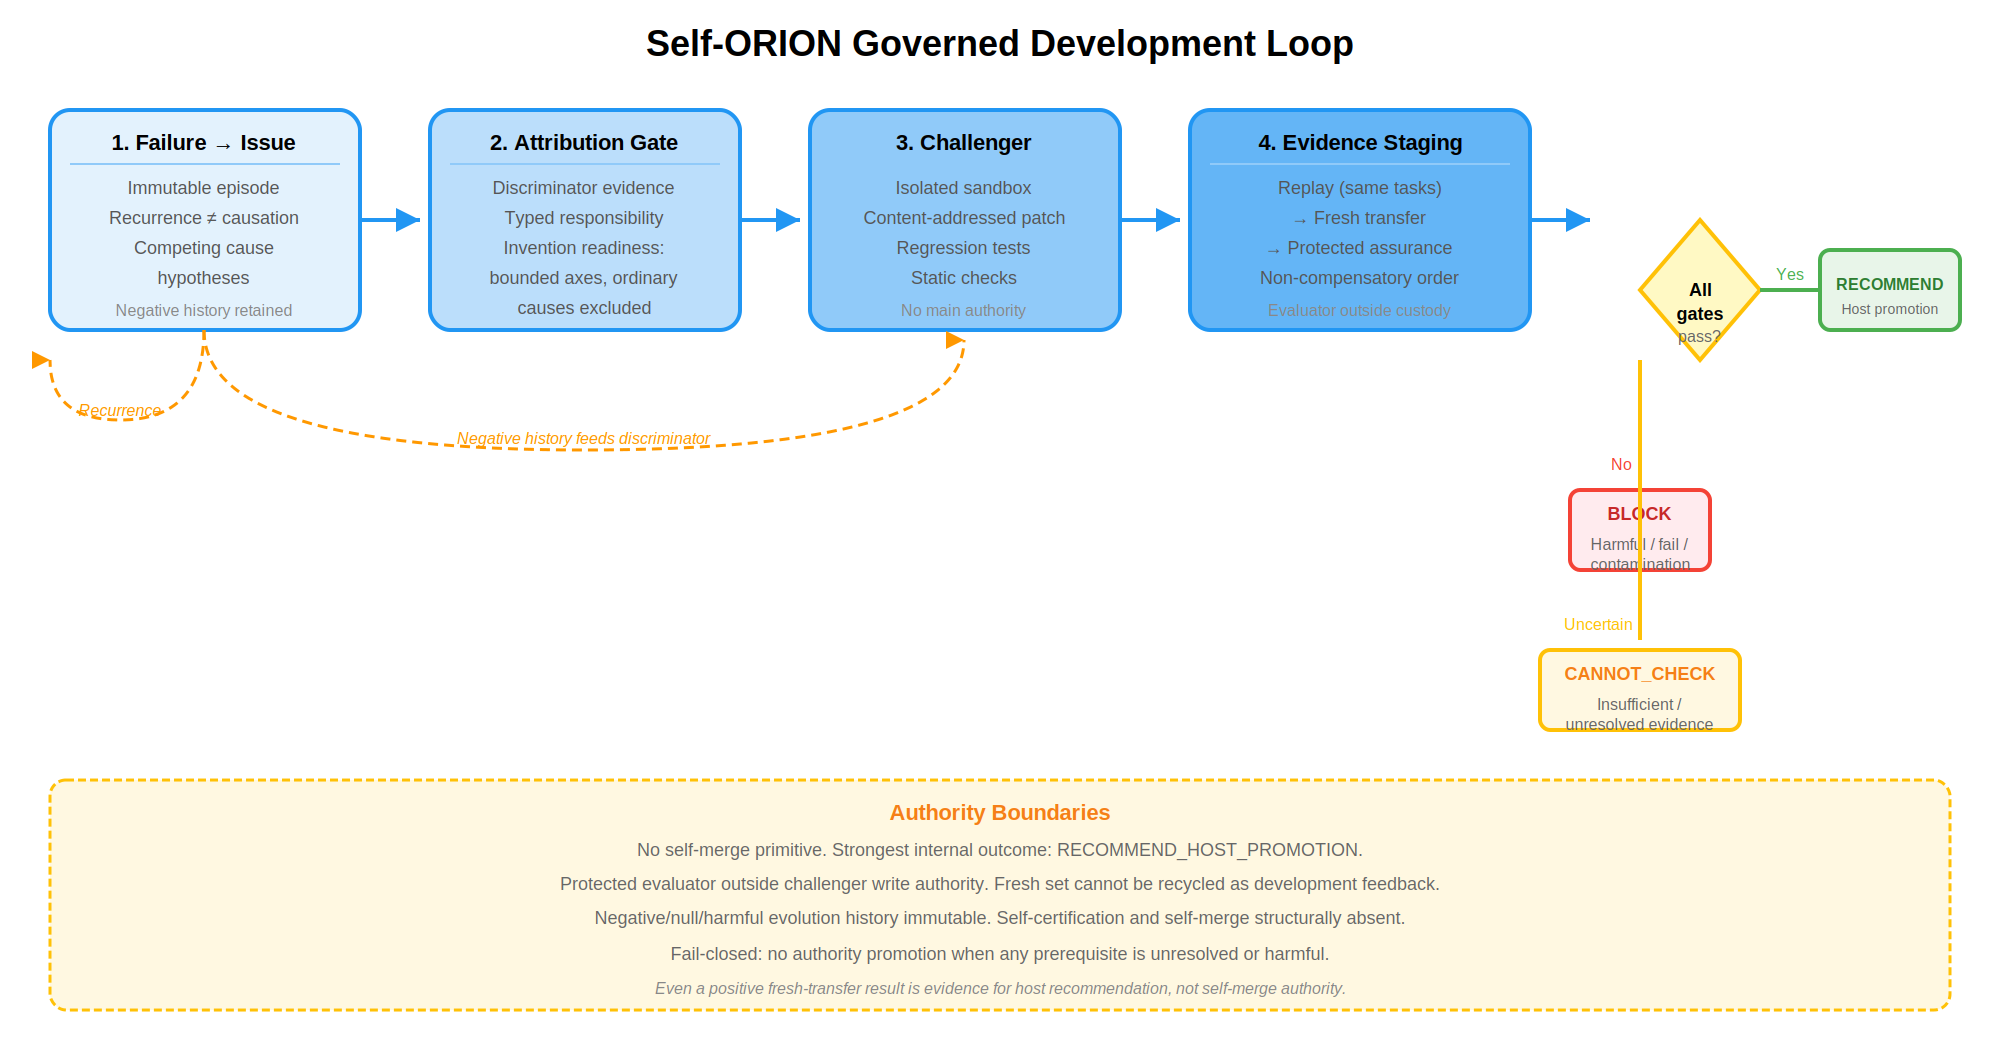
\includegraphics[width=\textwidth]{../figures/p5_1_governed_development_loop.png}
  \caption{The governed development loop. The failure-to-method path proceeds through persistent issue recording, causal discrimination, invention-readiness gating, isolated challenger execution, non-compensatory evidence staging (replay $\rightarrow$ fresh transfer $\rightarrow$ protected assurance), and a fail-closed authority boundary. The strongest internal outcome is a host recommendation; self-merge and self-certification are structurally absent.}
  \label{fig:P5-1}
\end{figure}

A method-evolving research system must answer three different questions: what
latent defect produced the observation, what is the least method revision that
the available evidence licenses, and who is allowed to conclude that the
revision is better. Collapsing the first two turns a recurring symptom into an
unlicensed broad rewrite. Collapsing the last two creates a self-promotion
channel. A coding agent may produce an impressive patch, but if it can also
rewrite the benchmark, choose only favorable episodes, change protected
governance, or certify its own evidence, improvement is not established.

Development is therefore treated here as an evidence-governed research process
rather than as a direct self-edit loop. The empirical claim under test is
narrower than ``autonomous self-improvement'', but the analytic question is
broader than one architecture:

\begin{quote}
Failures may become method knowledge only after persistent recording, causal discrimination, nearest-work/transfer challenge, isolated challenger execution, replay, fresh transfer and protected assurance; the candidate process cannot grant itself method authority or merge its own change.
\end{quote}

A method state is not writable merely because a research run failed. A failure
first changes the evidence available \emph{about} the method.
Section~\ref{sec:minimal-revision-theory} shows that a revision can be identified
only when the observed evidence and interventions separate every latent
situation requiring a different minimal front. Only a separately governed
transition can change which method is authorized.

\subsection{Contributions}

Four contributions carry the argument, and each is a property of the theory or
mechanism rather than of any particular system that implements it:

\begin{enumerate}
  \item a revision-factorization theorem and arbitrary-loss Bayes bound for
  method revision under observational equivalence;
  \item a discriminator-cover theorem that converts every unresolved
  cross-revision collision into an explicit intervention-design problem;
  \item a failure-to-method path that separates observation, recurrence,
  attribution, minimal revision, challenger construction and authority; and
  \item non-self-promotional evolution with isolated execution, protected fresh
  assurance, immutable adverse history and final promotion in external host
  custody.
\end{enumerate}

The factorization and Bayes identities are standard mathematical consequences
made operational here for revision-level selection; they are not claimed as
new general decision theory. The discriminator-cover reduction, typed revision
target and non-self-promotion consequence form the paper's theoretical
composition. None establishes empirical superiority. Section~\ref{sec:related}
places each component among its neighbours, and Section~\ref{sec:limitations}
states what the present evidence does and does not support.
